\section{Reducing the MPI grid setup and initial load balancing overhead}


\chapterDescription
  {
    Around 30 minutes.
  }
  {
    A working MPI code.
  }


In this section, we assume that you've a reasonable load balancing and that you
were able to postprocess your performance analysis outputs. We discuss 


\paragraph{The smell}

\begin{center}
  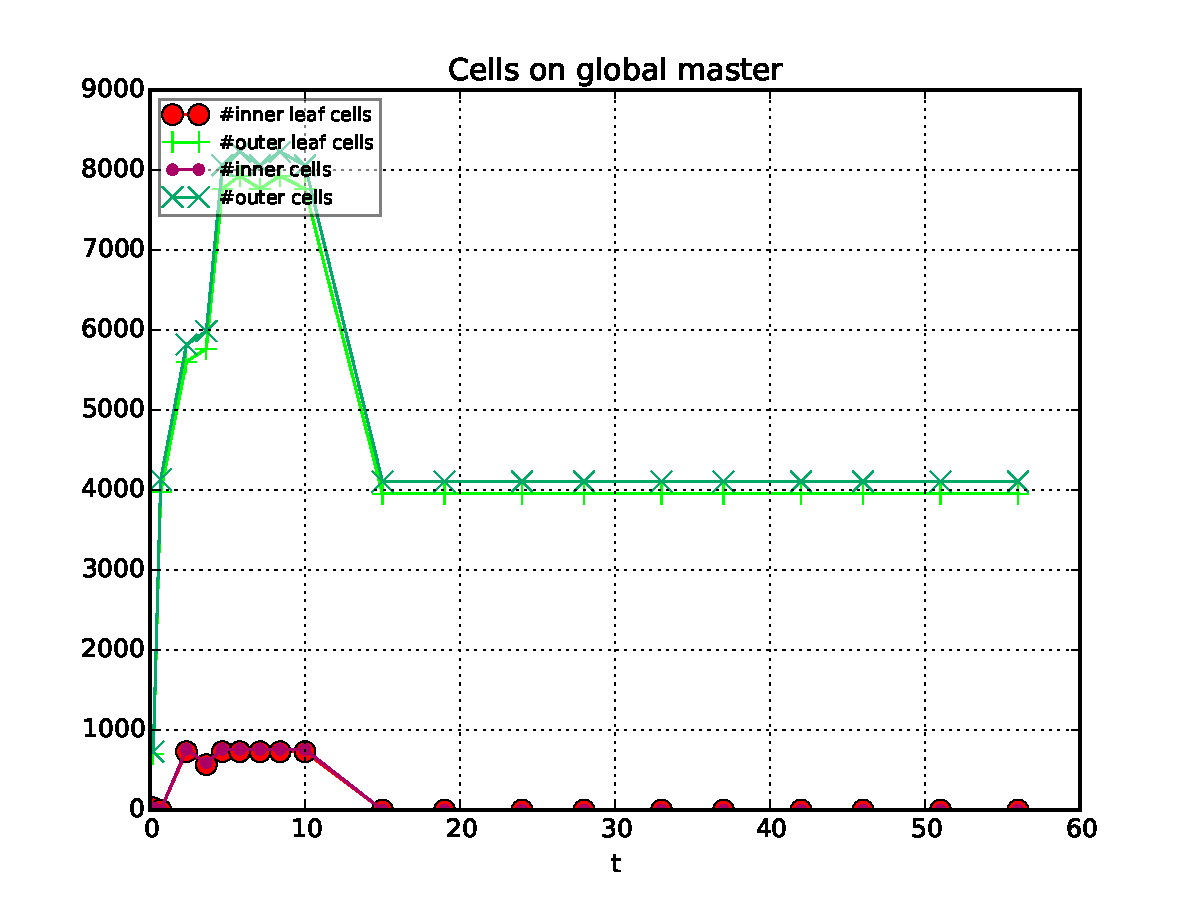
\includegraphics[width=0.5\textwidth]{41_mpi-setup/performance-analysis-output.pdf}
\end{center}



If you identify ranks whose local load decreases incrementally, these are ranks
that step by step fork more of their work to other ranks. 
In principle, this is fine and a result of load balancing. 
For reasonably static setups, it however is irritating: 
why is there such a long setup phase where obviously solely data is
redistributed?

The reason can be found in the semantics of \texttt{createVertex} and
\texttt{touchVertexFirstTime}.
Both operations try to refine the grid around the respective vertex immediately. 
Only if circumstances such as a parallel partitioning running through this
vertex---the refinement instruction then first has be distributed to all ranks
holding a copy of this vertex---do not allow Peano to realise the refinement
immediately, the refinement is postponed to the next iteration.
In many parallel codes, all the refinement calls pass through immediately on
rank 0 before it can spawn any rank.
This leads to the situation that the whole grid is in one sweep built up on the
global master and afterwards successively distributed among the ranks.


Such a behaviour is problematic: the global rank might run out of memory, lots
of data is transferred, and the sweeps over the whole grid on rank 0 are
typically pretty expensive. 
A distributed grid setup is advantageous.

\paragraph{The solution}

To facilitate this, it makes sense to switch from an aggressive
refinement into an iterative grid refinement strategy (one refinement level per
step, e.g.) to allow the rank to deploy work throughout the grid construction
and thus build up the grid in parallel and avoid the transfer of whole grid
blocks due to rebalancing.
Simply move your \texttt{refine()} call from the creational or touch first
events into \texttt{touchVertexLastTime()}:
As a consequence, setting up a (rather regular) grid of depth k requires at least k iterations. 


To find out when a grid has been constructed and balanced completely, the
repository provides an operation. Instead of writing something along the lines

\begin{code}
  repository.switchToSetup();
  repository.iterate();
\end{code}

\noindent
you have to write
\begin{code}
  repository.switchToSetupExperiment();
  do {
    repository.iterate();
  } while ( !repository.getState().isGridBalanced() );
\end{code}



\paragraph{Related pitfalls \& ideas}

As always, the devil is in the details:
\begin{itemize}
  \item  For many load balancing algorithms, it does make sense to create an
  initial grid of depth $\hat k <k$ on your rank 0 before you do any load
  balancing. This allows the load balancing metric to get a first idea about
  what the grid will look like and then to trigger an appropriate load
  balancing. To do so, you can require two mappings: one that builds up the grid
  in \texttt{createVertex} and \texttt{touchVertexFirstTime} up to a certain
  finest level, and one additional mapping that incrementally creates the
  additional mappings and thus allows for a fine-tuned load balancing.
  \item Once all ranks have obtained `their' partition, it does not make sense
  to continue to build up at most one grid level per sweep. In this case, you
  have to reliase an inverse pattern compared to the pattern sketched in the
  first bullet point.
  \item Everytime you rebalance your grid, Peano disables dynamic load balancing
  for a couple of iterations (three or four). Throughout these iterations, it
  can recover all adjacency information if the grid itself changes as well.
  Consequently, it does make sense to add a couple of adapter runs after each
  grid modification that to not change the grid structure: When you know that
  you have an adapter that changes the grid, apply afterwards an adapter that
  does not change the grid for a couple of times. This way, you ensure that no
  mpi rank runs out of memory. The grid generation does not overtake the rebalancing.
  \item If you are using the heap data structure, it furthermore makes sense to split up
the initialisation into a grid setup and a data struture initialisation.
You balance and distribute the grid setup following the recommendations above
and then in one additional sweep initialise the heap.
You initialise the heap as late as possible and thus avoid unneccesary
administrative overhead.
\end{itemize}
